%----------------------------------------------------------------------------------------
%   TITLE SECTION
%----------------------------------------------------------------------------------------
\newcommand{\horrule}[1]{\rule{\linewidth}{#1}} % Create horizontal rule command with 1 argument of height

\begin{titlepage}

\begin{center}
\begin{figure}[htpb]
    \begin{center}
        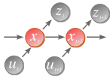
\includegraphics[width = 0.3\textwidth]{logo.png} % Just THIS!!!
    \end{center}
\end{figure}

\vspace*{10mm}
\normalfont\large
\texttt{MRPT}\\
Mobile Robot Programming Toolkit\\
Version: \MRPTVERSION

\vspace*{10mm}

\horrule{0.5pt} \\[0.4cm] % Thin top horizontal rule
\LARGE graphslam-engine: execute graphSLAM using rawlog files in MRPT
\horrule{2pt} \\[0.5cm] % Thick bottom horizontal rule
\vspace*{10mm}

\normalfont\large
Nikos Koukis\\
nickkouk@gmail.com\\
National Technical University of Athens\\
\vspace*{10mm}
\vfill

Document build: \today


\end{center}
\end{titlepage}
